\documentclass[notes]{subfiles}
\begin{document}
	\addcontentsline{toc}{section}{3.6 - The Chain Rule}
	\refstepcounter{section}
	\fancyhead[RO,LE]{\bfseries \nameref{cs36}} 
	\fancyhead[LO,RE]{\bfseries \small \currentname}
	\fancyfoot[C]{{}}
	\fancyfoot[LO,RE]{\large \thepage}	%Footer on Right \thepage is pagenumber
	\fancyfoot[RO,LE]{\large Chapter 3.6}
	
\section*{The Chain Rule}\label{cs36}
	\subsection*{Before Class}
	\subsubsection*{Review: Function Composition}
		\begin{ex}
			If \(f(u)= \sqrt{u}\) and \(u(x) = x^2 + 1\), find the composition \((f\circ u)(x)\).
		\end{ex}
			\vs{1}
			
		\begin{ex}
			Let \(k(x) = \cos 2x\).  Find two functions \(f,g\) such that \(k(x) = f(g(x))\).
		\end{ex}
			\vs{1}
			
		\begin{ex}
			Let \(f(x) = \sec^2 (x^2 + 9)\).  Find functions \(a,b,c\) such that \(f(x) = (a\circ b\circ c)(x)\)
		\end{ex}
			\vs{1}
			\newpage
			
	\subsubsection*{The Chain Rule}
		The chain rule \emph{relies} on being able to decompose a function into smaller pieces, and doing things in the right order.  
		\begin{thm}[Chain Rule]
			If \(g\) is differentiable at \(x\), and \(f\) is differentiable at \(g(x)\), then the composite function \(F = f\circ g\) defined by \(F(x) = f(g(x))\) is differentiable at \(x\), and\\[25pt] \vspace*{45pt}
			
			In Leibniz notatation, if \(y = f(u)\) and \(u = g(x)\) are both differentiable functions, then\\ \[\]\vspace*{50pt}
			
		\end{thm}

		\begin{ex}
			Let \(k(x) = \cos 2x\).  Find \(k'(x)\) using Example 3.6.2.
		\end{ex}
			\vs{1}
		
		\begin{ex}
			Let \(g(x) = \sin 4x\).  Find \(g'(x)\).
		\end{ex}
			\vs{1}
			\newpage
			
		\begin{ex}
			Let \(f(x) = \sec^2(x^2+9)\).  Use Example 2.5.3 to find \(f'(x)\).
		\end{ex}
			\vs{1}
			
		\begin{ex}
			Let \(g(x) = \sqrt[3]{x^2 + 5x}\).
			\begin{enumerate}[(a)]
				\item Why do we need to use the chain rule to compute this derivative?
					\vs{.5}
					
				\item Find \(f'(x)\).
					\vs{1}
					
				\item Find \(f''(x)\)
					\vs{2}
			\end{enumerate}
		\end{ex}
			\newpage
			
	\subsection*{Pre Class Practice}		
		\begin{ex}
			You are given a composite function.  Identify the inner function $u = g(x)$ and the outer function $y = f(u)$.
			\begin{enumerate}[(a)]
				\item \( \sqrt[3]{1+4x}\)
					\vs{.5}
					
				\item \(\sin (\cot x)\)
					\vs{.5}
					
				\item \((5x^6 + 2x^3)^4\)
					\vs{.5}
			\end{enumerate}
		\end{ex}
		
		\begin{ex}
			Set \(h(x) = \sin (x^2)\).  Identify the inner function \(u = g(x)\) and the outer function \(y = f(u)\).  Then, find the derivative \(h'(x)\).
		\end{ex}
			\vs{1}
			
		\begin{ex}
			Set \(k(t) = \sin^2(t)\).  Identify the inner function \(u = g(t)\) and the outer function \(y = f(u)\).  Then, find the derivative \(k'(t)\).
		\end{ex}
			\vs{1}
			\newpage
			
	\subsection*{In Class}
	\subsubsection*{Examples}
		\begin{ex}
			Let \(f(x) = \sqrt{x^2 + 1}\).  Find \(f'(x)\).
		\end{ex}
			\vs{1.5}
			
		\begin{ex}
			Let \(g(x) = \cos (x^2)\).  Find \(g'(x)\).
		\end{ex}
			\vs{1.5}
			
		\begin{ex}
			Find the derivative of \(k(t) = (2t+1)^5(t^3-t+1)^4\)
		\end{ex}
			\vs{2}
			\newpage
			
		\begin{ex}
			Let \(h(x) = \sin^2(\sqrt{x^2-1})\).  Find \(h'(x)\).
		\end{ex}
			\vs{2}
			
		\begin{ex}
			Find the first derivative of \(F(x) = (5x^5+2x^3)^4\)
		\end{ex}
			\vs{1}
			
		\begin{ex}
			Find the first derivative of \(h(t) = (2-\sin t)^{3/2}\)
		\end{ex}
			\vs{1}
			
		\begin{ex}
			Find the first derivative of \(y=\dfrac{1}{(\cos t + \tan t)^2}\)
		\end{ex}
			\vs{1}
			\newpage
		\begin{ex}
			Find the first derivative of \(h(\theta) = \tan (\theta^2\sin\theta)\)
		\end{ex}
			\vs{1}
			
		\begin{ex}
			Find the first derivative of \(y=\lrpar{\dfrac{1-\cos 2x}{1+\sin 2x}}^3\)
		\end{ex}
			\vs{1}
			
		\begin{ex}
			Find the first derivative of \(f(t) = \sqrt{t+\sqrt{t}}\)
		\end{ex}
			\vs{1}
			\newpage
			
		\begin{ex}
			Find the first derivative of \(r(x) = (x^2+1)^3(x^2+2)^6\)
		\end{ex}
			\vs{1}
			
		\begin{ex}
			Find the first derivative of \(y = \sqrt[5]{\dfrac{x}{x-1}}\)
		\end{ex}
			\vs{1}
			
		\begin{ex}
			Find the first derivative of \(z = \sqrt{\sin(1+x^2)}\)
		\end{ex}
			\vs{1}
			\newpage
			
		\begin{ex}
			Find the first derivative of \(A(t) = \dfrac{t^2}{\sqrt{t^3+1}}\)
		\end{ex}
			\vs{1}
			
		\begin{ex}
			Find the first derivative of \(f(x) = \cos^4(\tan^3(x))\)
		\end{ex}
			\vs{2}
			
		\begin{ex}
			Find the first derivative of \(y = \cos\sqrt{\sin(\tan\pi x)}\)
		\end{ex}
			\vs{2}
			\newpage
			
		\begin{ex}
			Find an equation of the tangent line to the curve \(y = \sqrt{1+x^3}\) at the point \((2,3)\)
		\end{ex}
			\vs{1}
			
		\begin{ex}
			Let \(f(x) = [g(\cos x)]^2\).  Write an expression for \(f'(x)\).
		\end{ex}
			\vs{1}
			
		\begin{ex}
			If \(h(x) = \sqrt{4+3f(x)}\), \(f(1) = 7\), and \(f'(1) = 4\), find \(h'(1)\).
		\end{ex}
			\vs{1}
			
		\begin{ex}
			If \(g(x) = \sqrt{f(x)}\), where \(f\) is the function shown, evaluate \(g'(3)\).\\
			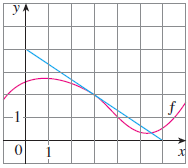
\includegraphics{3.6fig1}
		\end{ex}
			\vs{.25}
			\newpage
		
		\begin{ex}
			A table of values for \(f,g,f'\), and \(g'\) is given:
			\begin{center}
				\begin{tabular}{|c|c|c|c|c|}\hline
					\(x\)	& \(f(x)\)	& \(g(x)\)	& \(f'(x)\)	& \(g'(x)\) \\ \hline
					1 & 3 & 2 & 4 & 6\\
					2 & 1 & 8 & 5 & 7\\
					3 & 7 & 2 & 7 & 9\\ \hline
				\end{tabular}
			\end{center}
			\begin{enumerate}[(a)]
				\item Find \(h'(1)\), if \(h(x) = f(g(x))\)
					\vs{.5}
					
				\item Find \(H'(1)\), if \(H(x) = g(f(x))\)
					\vs{.5}
			\end{enumerate}
		\end{ex}
		
		\begin{ex}
			Find the first and second derivatives of \(y = \sin (\cos 4\theta)\)
		\end{ex}
			\vs{2}
			\newpage
			
	\subsection*{After Class Practice}
		\begin{ex}
			Find the first and second derivatives of \(y = \dfrac{4x}{\sqrt{x+1}}\)
		\end{ex}
			\vs{1}
		\begin{ex}
			Find \(D^{35} \sin \pi x\)
		\end{ex}
			\vs{1}
		
		\begin{ex}
			Suppose \(f\) is differentiable on \(\R\), and \(A\) is a real number.  Let \(F(x) = f(x^A)\) and \(G(x) = [f(x)]^A\).  Find expressions for \(F'(x)\) and \(G'(x)\).
		\end{ex}
			\vs{1}
			
		\begin{ex}
			The chain rule is often a source of confusion and frustration for students in (and beyond) calculus.  What do you think will help the chain rule stick out in your mind?
		\end{ex}
			\vs{1}

\clearpage
\end{document}
